\PassOptionsToPackage{dvipsnames}{xcolor}
\documentclass[10pt, xcolor={usenames, dvipsnames}]{beamer}

\usepackage[scale=2]{ccicons}
\usepackage{graphicx}
\usepackage{booktabs}
\usepackage{gensymb}
\usepackage{multimedia}
\usepackage{hyperref}
\usepackage{txfonts}
\usepackage{caption}
\usepackage{subcaption}

% Beamer configuration
\usetheme[sectionpage=progressbar, numbering=counter, progressbar=frametitle]{metropolis}

\usepackage{pgfplots}
\usepackage{pgfplotsthemetol}
\usepackage{tikz}
\usetikzlibrary{positioning,arrows,decorations.pathmorphing,calc}

% Progressbar
\setbeamercolor{progress bar}{
    fg=TolLightGreen,
    bg=TolLightGreen!50!black!30
}
\makeatletter
    \setlength{\metropolis@titleseparator@linewidth}{2pt}
    \setlength{\metropolis@progressonsectionpage@linewidth}{2pt}
    \setlength{\metropolis@progressinheadfoot@linewidth}{2pt}
\makeatother

% Footer
\setbeamertemplate{frame footer}{Quentin Brateau, ENSTA Bretagne}

% Block fill
\metroset{block=fill}

\title{Torpedo-like AUV control in constrained environment}
\date{\today}
\author{Quentin Brateau}
\institute{ENSTA Bretagne}

\titlegraphic{
    \centering
    \begin{tabular}{lllll}
        \href{https://www.defense.gouv.fr/aid}{
\includegraphics[height=0.6cm]{imgs/logo_aid}} &
        \href{https://www.gdr-robotique.org/}{
\includegraphics[height=0.6cm]{imgs/logo_gdr}} &
        \href{https://www.ensta-bretagne.fr/fr/}{
\includegraphics[height=0.6cm]{imgs/logo_ensta}} &
        \href{https://labsticc.fr/fr}{
\includegraphics[height=0.6cm]{imgs/logo_labsticc}} &
        \href{https://www.ensta-bretagne.fr/robex/}{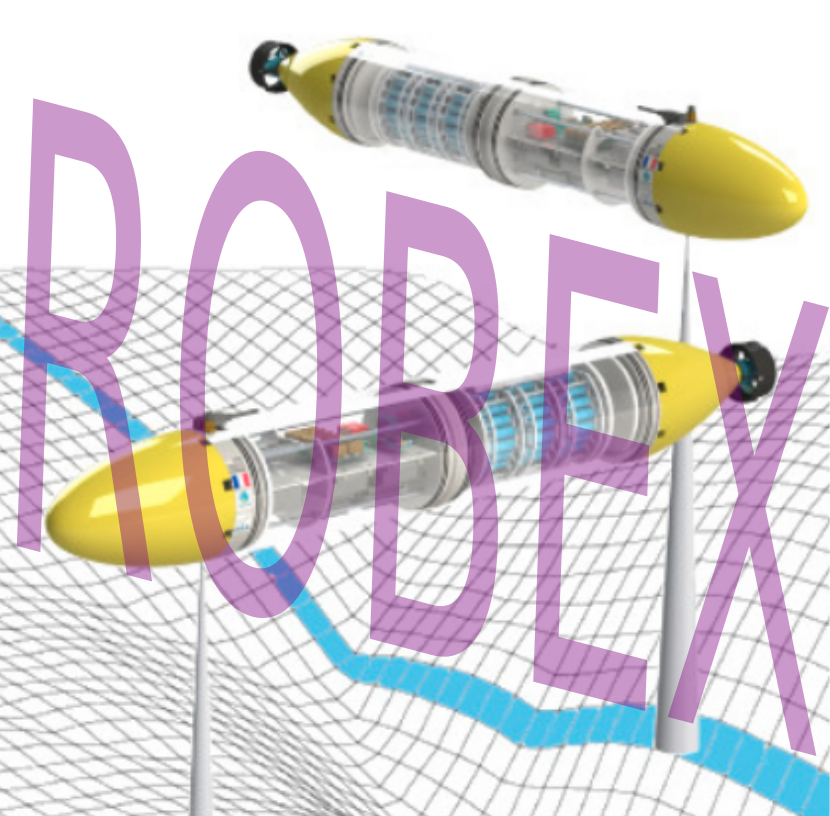
\includegraphics[height=0.6cm]{imgs/logo_robex}}
    \end{tabular}
}

\addtobeamertemplate{frametitle}{}{%
    \begin{tikzpicture}[remember picture,overlay]
    \node[anchor=north east,yshift=2pt] at (current page.north east) {
\includegraphics[height=0.9cm]{imgs/logo_ensta_bw}};
    \end{tikzpicture}
}

\begin{document}

    \maketitle

    % \begin{frame}{Table of contents}
    %     \setbeamertemplate{section in toc}[sections numbered]
    %     \tableofcontents[hideallsubsections]
    % \end{frame}

    \section{Context}

        \begin{frame}{Introduction}{PhD}
            \centering
            \begin{minipage}[c]{0.58\textwidth}
                \begin{block}{Research laboratory}
                    \vspace{0.2cm}
                    \begin{itemize}
                        \item ENSTA Bretagne, UMR 6285, Lab-STICC
                    \end{itemize}
                \end{block}

                \begin{block}{Supervisiors}
                    \begin{itemize}
                        \item Luc Jaulin
                        \item Fabrice Lebars
                    \end{itemize}
                \end{block}

                \begin{block}{Funding}
                    \begin{itemize}
                        \item AID funding: Jean-Daniel Masson
                    \end{itemize}
                \end{block}
            \end{minipage}
            \hfill
            \begin{minipage}[c]{0.4\textwidth}
                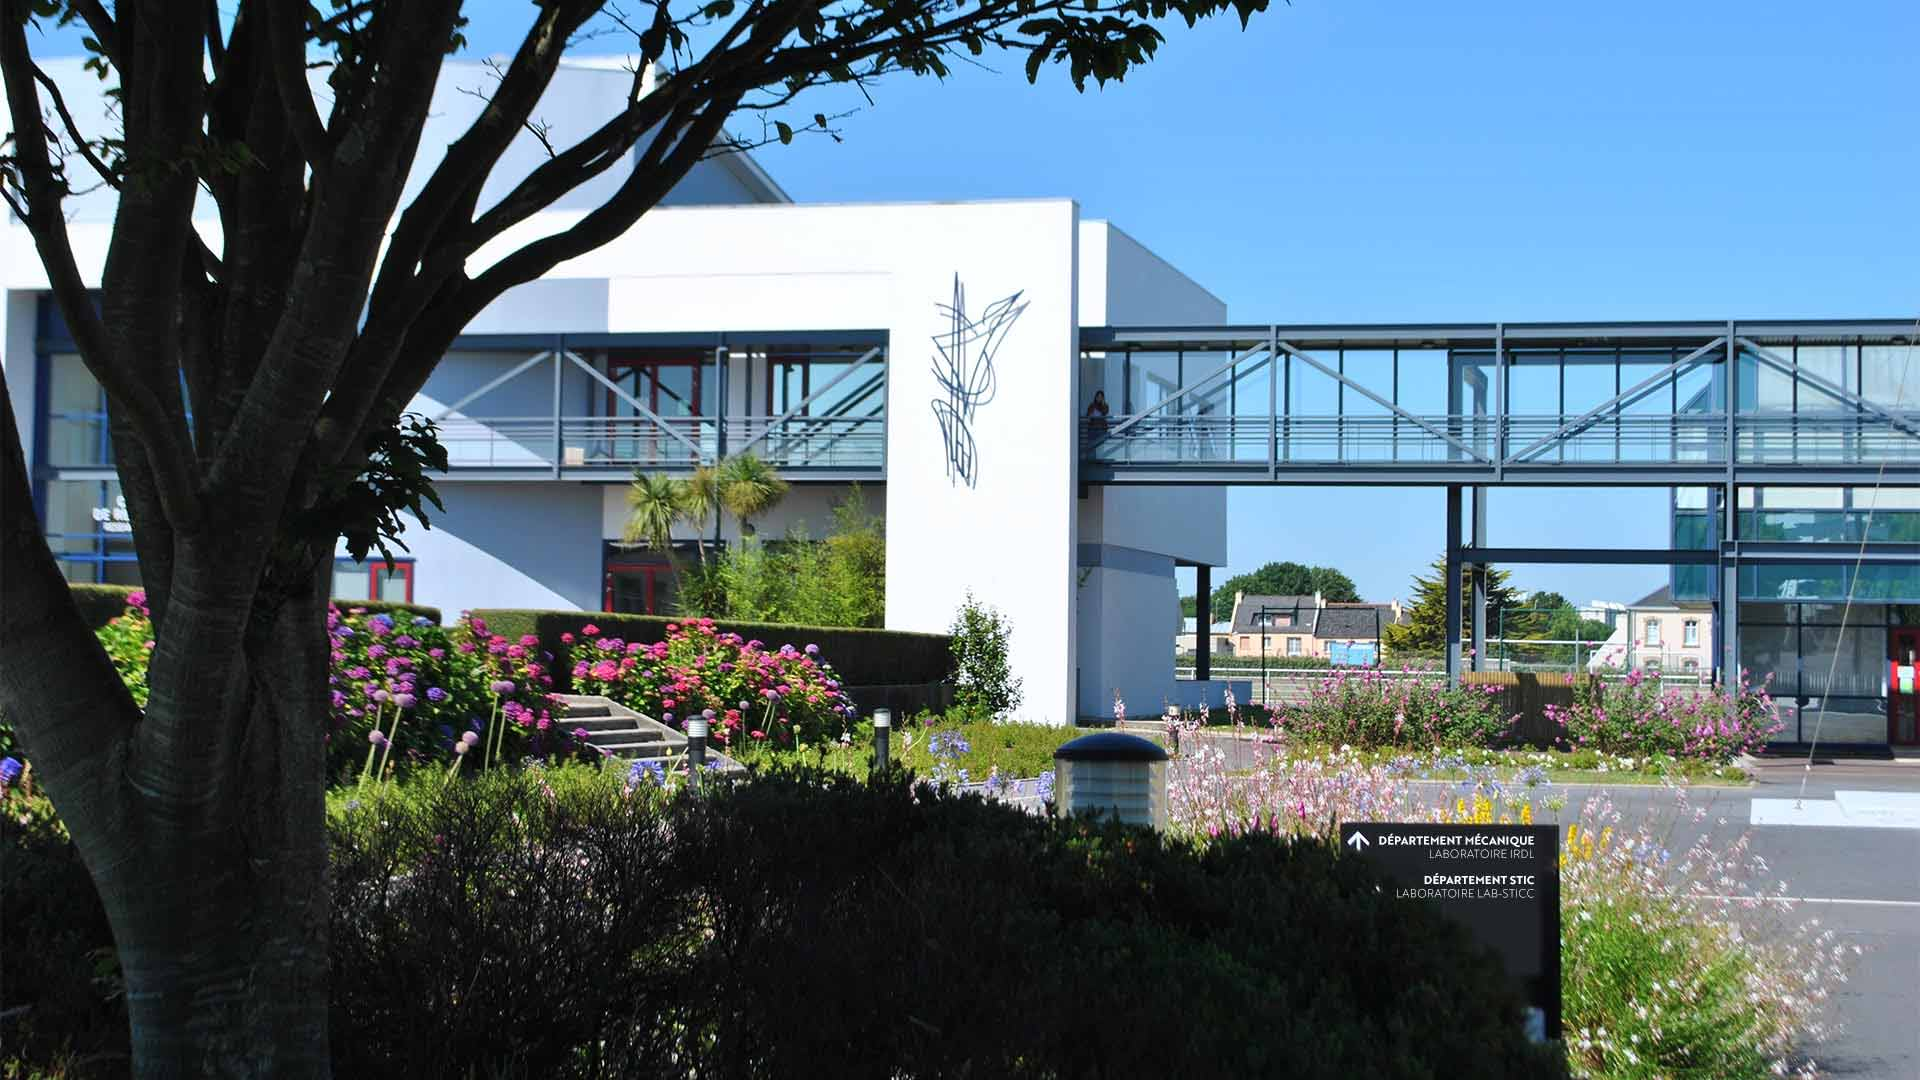
\includegraphics[height=0.7\textheight, trim={24cm 0 16cm 0}, clip]{imgs/ensta.jpg}
            \end{minipage}
        \end{frame}

        \begin{frame}{Introduction}
            \begin{minipage}[t]{0.55\textwidth}
                \begin{block}{AUV}
                    \vspace{0.25cm}
                    \begin{itemize}
                        \item Control of torpedo-like AUV \\ 
                        \item Riptide's micro-uuv
                    \end{itemize}
                \end{block}
                \begin{block}{Environment}
                    \begin{itemize}
                        \item Constrained environment \\ 
                        \item Pool, harbor, ...
                    \end{itemize}
                \end{block}
                \begin{block}{Goals}
                    \begin{itemize}
                        \item Reactivity \\
                        \item Manoeuvrability
                    \end{itemize}
                \end{block}
            \end{minipage}
            \hfill
            \begin{minipage}[t]{0.4\textwidth}
                \begin{figure}[htb]
                    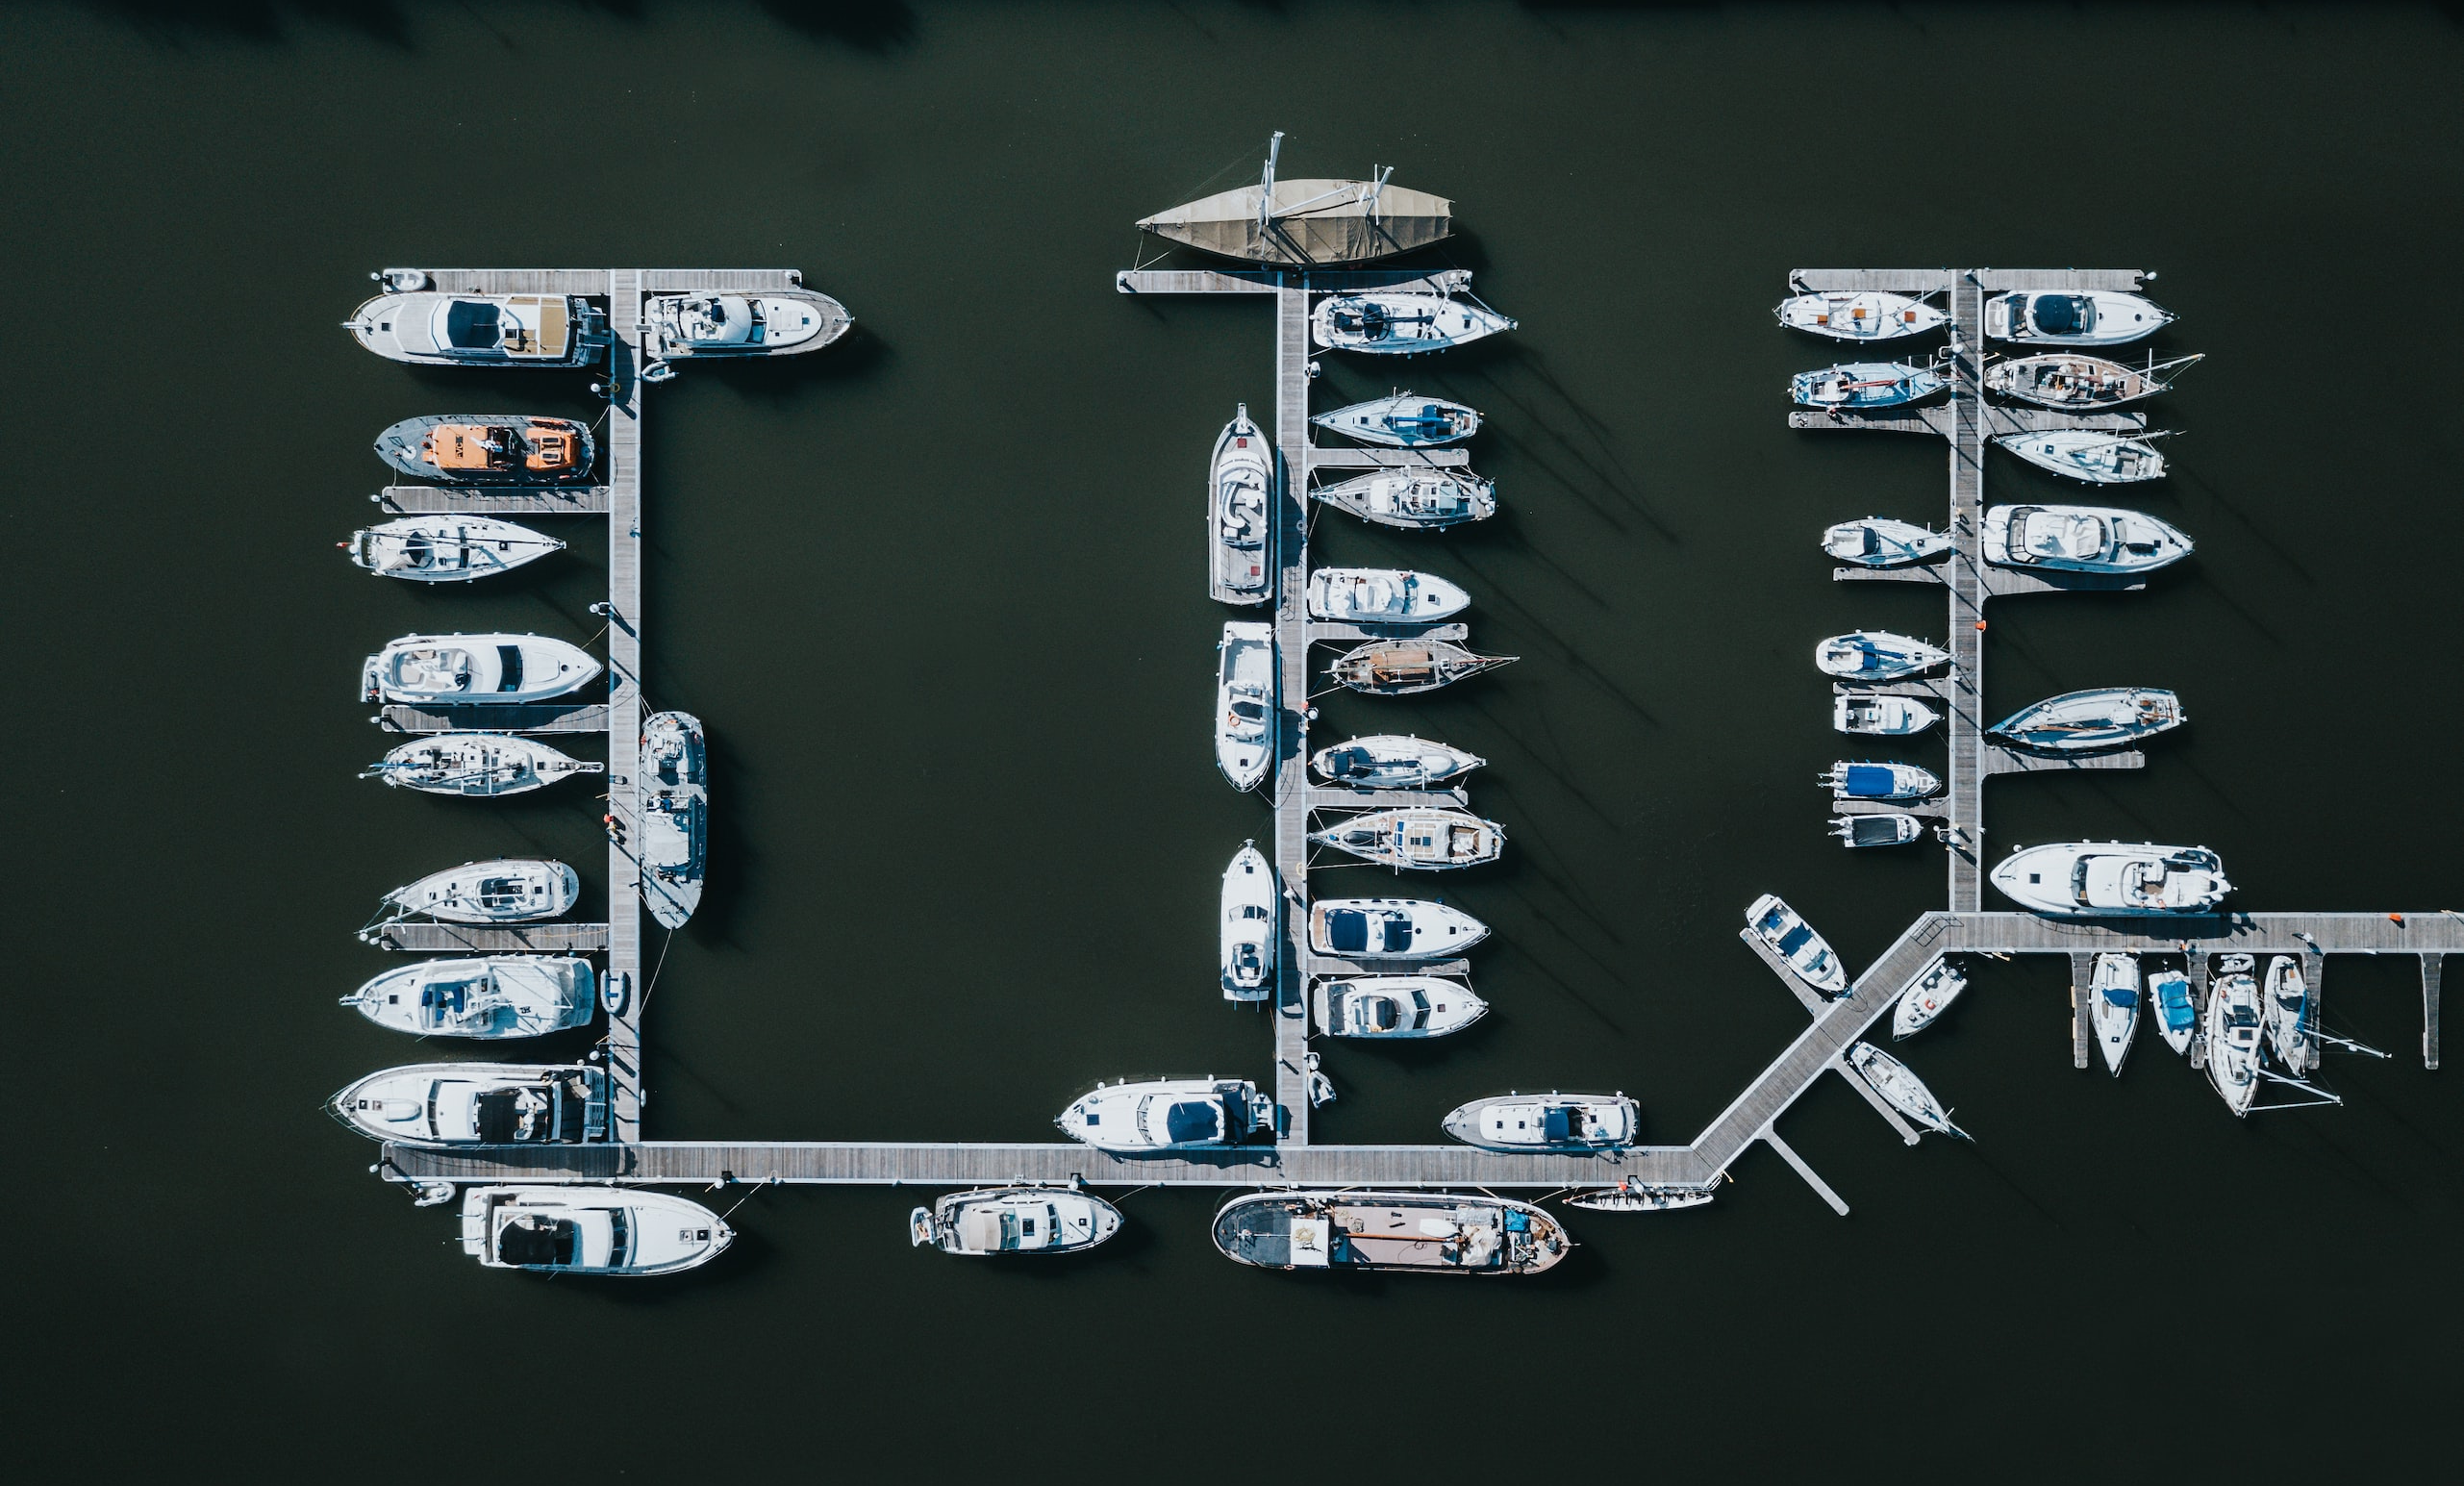
\includegraphics[width=\textwidth]{imgs/harbour.png}

                    \vspace{.1cm}

                    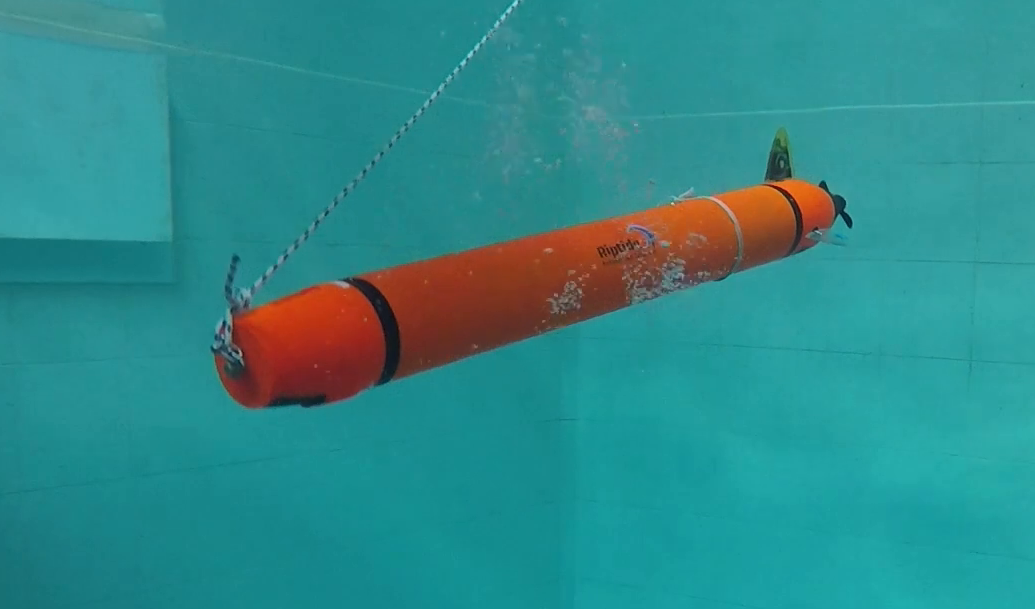
\includegraphics[width=\textwidth]{imgs/riptide.png}
                    \caption{Harbor and Riptide in the ENSTA Bretagne pool}
                \end{figure}
            \end{minipage}
        \end{frame}

    \section{Motivation}

        \begin{frame}{Obstacle avoidance}
            \begin{minipage}[b]{0.5\textwidth}
                \begin{block}{Wall avoidance}
                    \vspace{0.2cm}
                    \begin{itemize}
                        \item Sense wall \\
                        \item Determine normal vector $\mathbf{u}$ \\
                        \item Reorient AUV orthogonal to $\mathbf{u}$
                    \end{itemize}
                \end{block}
                \begin{block}{Control law}
                    \begin{itemize}
                        \item Without singularities \\
                        \item Based on reliable sensors \\
                        \item Independant of orientation \\
                        \item As fast as possible
                    \end{itemize}
                \end{block}
            \end{minipage}
            \hfill
            \begin{minipage}[b]{0.46\textwidth}
                \begin{figure}
                    \centering
                    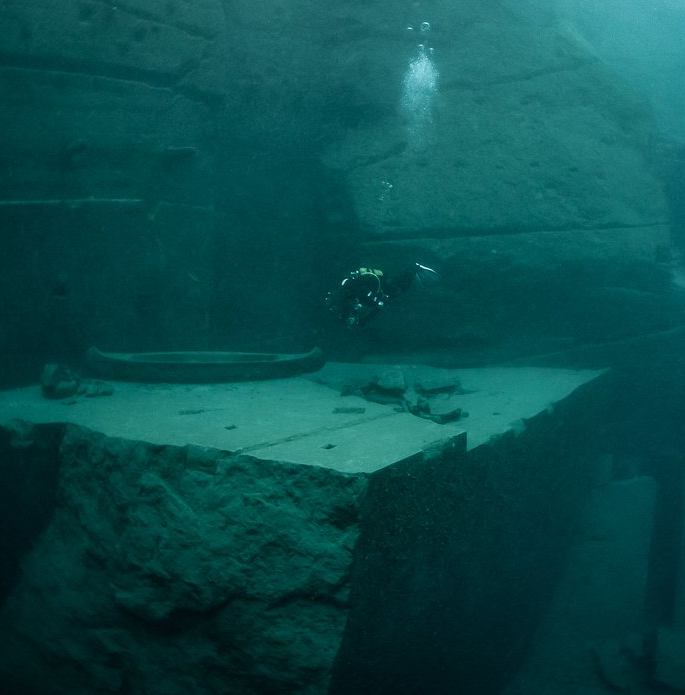
\includegraphics[width=0.95\textwidth]{imgs/vodelee.png}
                    \caption{Vodelée Career - Belgium}
                \end{figure}
            \end{minipage}
        \end{frame}

        \begin{frame}{Classical control}
            \centering
            \begin{minipage}{0.45\textwidth}
                \centering
                \begin{figure}
                    \begin{tikzpicture}
                        \shade[ball color = gray!40, opacity = 0.4] (0,0) circle (2cm);
                        \draw[thick] (0,0) circle (2cm);
                        \onslide<2->{
                            \coordinate (R1) at (0.8,1.3);
                            \draw[thick,red,->,>=latex] (0,0) -- node[midway,above left] {$\mathbf{u}$} (R1); 
                        }
                        \onslide<3->{
                            \coordinate (R2) at (-0.2,1.15);
                            \draw[thick,ForestGreen,->,>=latex] (0,0) -- node[midway,above left] {$\mathbf{v}$} (R2); 
                        }
                        \onslide<4->{
                            \begin{scope}[rotate around={-30:(0,0)}]
                                \draw[thick] (-2,0) arc (180:360:2 and 0.6) coordinate[pos=0.2] (R3);
                                \draw[dashed] (2,0) arc (0:180:2 and 0.6);
                            \end{scope}
                            \draw[thick,RoyalBlue,->,>=latex] (0,0) -- node[midway,above] {$u_\bot$} (R3);
                            }
                        \onslide<5-> {
                            \path[thick,->,>=latex,RoyalPurple] (R2) edge[in=60,out=160] (R3);
                            \coordinate[below right=1.2mm and 1.2mm of R3] (R4);
                            % \draw[thick,->,>=latex,RoyalPurple] (R4) arc (-45:-225:2mm);
                        }
                    \end{tikzpicture}
                    \caption{Representation in $S^2$}
                \end{figure}
            \end{minipage}
            \begin{minipage}{0.45\textwidth}
                \centering
                \begin{figure}
                    \begin{tikzpicture}
                        \shade[ball color = gray!40, opacity = 0.4] (0,0) circle (2cm);
                        \draw[thick] (0,0) circle (2cm);
                        \onslide<2->{
                            \coordinate (R1) at (0.8,1.3);
                            \node[red] at (R1) {$\bullet$} node[red] at (R1) [below right] {$\mathbf{R}_u$};
                        }
                        \onslide<3->{
                            \coordinate (R2) at (-0.2,1.15);
                            \node[ForestGreen] at (R2) {$\bullet$} node[ForestGreen] at (R2) [above] {$\mathbf{R}_v$};
                        }
                        \onslide<4->{
                            \begin{scope}[rotate around={-30:(0,0)}]
                                \draw[thick] (-2,0) arc (180:360:2 and 0.6) coordinate[pos=0.2] (R3);
                                \draw[dashed] (2,0) arc (0:180:2 and 0.6);
                            \end{scope}
                            \node[thick,RoyalBlue] at (R3) {$\bullet$} node[RoyalBlue] at (R3) [below] {$\mathbf{R}_{u_\bot}$};
                        }
                        \onslide<5->{
                            \path[thick,->,>=latex,RoyalPurple] (R2) edge[in=60,out=160] node[midway,below] {$R_w$} (R3);
                        }
                    \end{tikzpicture}
                    \caption{Representation in $SO(3)$}
                \end{figure}
            \end{minipage}
        \end{frame}

        \begin{frame}{Classical control}
            \centering
            \begin{minipage}{0.75\textwidth}
                \begin{block}{Strengths}
                    \vspace{0.2cm}
                    \begin{itemize}
                        \item Often already implemented for other purposes
                        \item AUV orientation fully controlled
                    \end{itemize}
                \end{block}
                \begin{block}{Weaknesses}
                    \begin{itemize}
                        \item AUV angles have to be known
                        \item Not the quickest reorientation
                        \item Set all angles
                    \end{itemize}
                \end{block}
            \end{minipage}
        \end{frame}

        \begin{frame}{Proposed approach}
            \centering
            \begin{minipage}{0.45\textwidth}
                \centering
                \begin{figure}
                    \begin{tikzpicture}
                        \shade[ball color = gray!40, opacity = 0.4] (0,0) circle (2cm);
                        \draw[thick] (0,0) circle (2cm);
                        \onslide<2->{
                            \coordinate (R1) at (0.8,1.3);
                            \draw[thick,red,->,>=latex] (0,0) -- node[midway,above left] {$\mathbf{u}$} (R1); 
                        }
                        \onslide<3->{
                            \coordinate (R2) at (-0.2,1.15);
                            \draw[thick,ForestGreen,->,>=latex] (0,0) -- node[midway,above left] {$\mathbf{v}$} (R2); 
                        }
                        \onslide<4->{
                            \begin{scope}[rotate around={-30:(0,0)}]
                                \draw[thick] (-2,0) arc (180:360:2 and 0.6) coordinate[pos=0.36] (R3) coordinate[pos=0.61] (R4);
                                \draw[dashed] (2,0) arc (0:180:2 and 0.6);
                            \end{scope}
                            \draw[thick,dotted] (R1) edge[in=30,out=175] (R2);
                            \draw[thick,RoyalBlue,->,>=latex] (0,0) -- node[midway,above] {$\mathbf{v_\bot}$} (R3);
                        }
                        \onslide<4>{
                            \draw[thick,dotted] (R2) edge[in=70,out=210] (R3);
                        }
                        \onslide<5->{
                            \path[thick,->,>=latex,RoyalPurple] (R2) edge[in=70,out=210] (R3);
                            \draw[thick,RoyalPurple,->,>=latex] (0,0) -- node[midway,right] {$\mathbf{w}$} (R4);
                        }
                    \end{tikzpicture}
                    \caption{Representation in $S^2$}
                \end{figure}
            \end{minipage}
            \begin{minipage}{0.45\textwidth}
                \centering
                \begin{figure}
                    \begin{tikzpicture}
                        \shade[ball color = gray!40, opacity = 0.4] (0,0) circle (2cm);
                        \draw[thick] (0,0) circle (2cm);
                        \onslide<2->{
                            \coordinate (R1) at (0.8,1.3);
                            \node[red] at (R1) {$\bullet$} node[red] at (R1) [below right] {$\mathbf{R}_u$};
                        }
                        \onslide<3->{
                            \coordinate (R2) at (-0.2,1.15);
                            \node[ForestGreen] at (R2) {$\bullet$} node[ForestGreen] at (R2) [above left] {$\mathbf{R}_v$};
                        }
                        \onslide<4->{
                            \begin{scope}[rotate around={-30:(0,0)}]
                                \draw[thick] (-2,0) arc (180:360:2 and 0.6) coordinate[pos=0.36] (R3);
                                \draw[dashed] (2,0) arc (0:180:2 and 0.6);
                            \end{scope}
                            \node[thick,RoyalBlue] at (R3) {$\bullet$} node[RoyalBlue] at (R3) [below left] {$\mathbf{R}_{v_\bot}$};
                        }
                        \onslide<5->{
                            \path[thick,->,>=latex,RoyalPurple] (R2) edge[in=70,out=210] node[midway, left] {$R_w$} (R3);
                        }
                    \end{tikzpicture}
                    \caption{Representation in $SO(3)$}
                \end{figure}
            \end{minipage}
        \end{frame}

        \begin{frame}{Proposed approach}
            \centering
            \begin{minipage}{0.75\textwidth}
                \begin{block}{Strengths}
                    \vspace{0.2cm}
                    \begin{itemize}
                        \item Set only necessary angles
                        \item Other angles don't need to be known
                        \item Quickest reorientation
                    \end{itemize}
                \end{block}
                \begin{block}{Weaknesses}
                    \begin{itemize}
                        \item Chosen direction not controlled
                    \end{itemize}
                \end{block}
            \end{minipage}
        \end{frame}

    \section{Orthogonal control}

        \begin{frame}{Determine $\mathbf{v_\bot}$}
            \begin{minipage}{0.4\textwidth}
                \centering
                \begin{figure}
                    \begin{tikzpicture}
                        \shade[ball color = gray!40, opacity = 0.4] (0,0) circle (2cm);
                        \draw[thick] (0,0) circle (2cm);
                        \coordinate (R1) at (0.8,1.3);
                        \draw[thick,red,->,>=latex] (0,0) -- node[midway,above left] {$\mathbf{u}$} (R1);
                        \begin{scope}[rotate around={-30:(0,0)}]
                            \draw[thick] (-2,0) arc (180:360:2 and 0.6) coordinate[pos=0.36] (R3);
                            \draw[dashed] (2,0) arc (0:180:2 and 0.6);
                        \end{scope}
                        \coordinate (R2) at (-0.2,1.15);
                        
                        \draw[thick,ForestGreen,->,>=latex] (0,0) -- node[midway,left]  {$\mathbf{v}$} (R2);
                        \onslide<2> {
                            \coordinate (vu) at ($(0,0)!0.78!(R1)$);
                            \draw[thick,dotted] (vu) -- (R2);
                            \draw[thick,RoyalPurple,->,>=latex] (0,0) -- node[midway,right] {$\langle \mathbf{u}, \mathbf{v}\rangle \cdot \mathbf{u}$} (vu);
                        }
                        \onslide<3> {
                            \coordinate (vv) at ($(0,0)!0.72!(R3)$);
                            \draw[thick,RoyalPurple,->,>=latex] (vv) -- node[midway,left] {$\langle \mathbf{u}, \mathbf{v}\rangle \cdot \mathbf{u}$} (R2);
                            \draw[thick,RoyalBlue,->,>=latex] (0,0) -- node[midway,below right] {$\mathbf{v} - \langle \mathbf{u}, \mathbf{v}\rangle \cdot \mathbf{u}$} (vv);
                            }
                        \onslide<4> {
                            \draw[thick,RoyalBlue,->,>=latex] (0,0) -- node[midway,below right] {$\mathbf{v_\bot}$} (R3);
                        }
                    \end{tikzpicture}
                    \caption{Representation in $S^2$}
                \end{figure}
            \end{minipage}
            \hfill
            \begin{minipage}{0.55\textwidth}
                \begin{block}{Determine $\mathbf{v_\bot}$}
                    \begin{equation}
                        \mathbf{v_\bot} = \frac{\mathbf{v} - \langle \mathbf{u}, \mathbf{v}\rangle \cdot \mathbf{u}}{||\mathbf{v} - \langle \mathbf{u}, \mathbf{v}\rangle \cdot \mathbf{u}||}
                    \end{equation}
                \end{block}
                
            \end{minipage}
        \end{frame}

        \begin{frame}{Determine $\mathbf{R_w}$ - Classical way}
            \begin{minipage}{0.4\textwidth}
                \centering
                \begin{figure}
                    \begin{tikzpicture}
                        \shade[ball color = gray!40, opacity = 0.4] (0,0) circle (2cm);
                        \draw[thick] (0,0) circle (2cm);
                        \coordinate (R1) at (0.8,1.3);
                        \draw[thick,red,->,>=latex] (0,0) -- node[midway,above left] {$\mathbf{u}$} (R1);
                        \draw[thick,RoyalBlue,->,>=latex] (0,0) -- node[midway,above] {$\mathbf{v_\bot}$} (R3);
                        \begin{scope}[rotate around={-30:(0,0)}]
                            \draw[thick] (-2,0) arc (180:360:2 and 0.6) coordinate[pos=0.36] (R3) coordinate[pos=0.61] (R4);
                            \draw[dashed] (2,0) arc (0:180:2 and 0.6);
                        \end{scope}
                        
                        \onslide<1>{
                            \coordinate (R2) at (-0.2,1.15);
                            \draw[thick,ForestGreen,->,>=latex] (0,0) -- node[midway,above left] {$\mathbf{v}$} (R2); 
                            \draw[thick,dotted] (R1) edge[in=30,out=175] (R2);
                            \path[thick,->,>=latex,RoyalPurple] (R2) edge[in=70,out=210] (R3);
                            \draw[thick,RoyalPurple,->,>=latex] (0,0) -- node[midway,right] {$\mathbf{w}$} (R4);
                        }
                        \onslide<2>{
                            \draw[thick,ForestGreen,->,>=latex] (0,0) -- node[midway,below right] {$\mathbf{v}$} (R3);
                        }
                    \end{tikzpicture}
                    \caption{Representation in $S^2$}
                \end{figure}
            \end{minipage}
            \hfill
            \begin{minipage}{0.55\textwidth}
                \begin{block}{Determine $R_w$}
                    \begin{equation}
                        \begin{split}
                            \mathbf{w} &= \mathbf{v} \wedge \mathbf{v_\bot} \\
                            \alpha &= arccos(\mathbf{||w||}) \\
                            \mathbf{R_w} &= exp\left(\alpha\frac{\mathbf{w}}{\color<2>{red}{||\mathbf{w}||}}t\right)
                        \end{split}
                    \end{equation}
                \end{block}
                \begin{block}<2->{Issue}
                    \centering
                    What if $\mathbf{v} = \mathbf{v_\bot}$ ?
                \end{block}
            \end{minipage}
        \end{frame}

        \begin{frame}{Determine $\mathbf{R_w}$ - Codesido flavor}
            \begin{minipage}{0.4\textwidth}
                \centering
                \begin{figure}
                    \begin{tikzpicture}
                        \shade[ball color = gray!40, opacity = 0.4] (0,0) circle (2cm);
                        \draw[thick] (0,0) circle (2cm);
                        \coordinate (R1) at (0.8,1.3);
                        \draw[thick,red,->,>=latex] (0,0) -- node[midway,above left] {$\mathbf{u}$} (R1);
                        \draw[thick,RoyalBlue,->,>=latex] (0,0) -- node[midway,above] {$\mathbf{v_\bot}$} (R3);
                        \begin{scope}[rotate around={-30:(0,0)}]
                            \draw[thick] (-2,0) arc (180:360:2 and 0.6) coordinate[pos=0.36] (R3) coordinate[pos=0.61] (R4);
                            \draw[dashed] (2,0) arc (0:180:2 and 0.6)  coordinate[pos=0.36] (R5);
                        \end{scope}
                        
                        \onslide<1-2>{
                            \coordinate (R2) at (-0.2,1.15);
                            \draw[thick,ForestGreen,->,>=latex] (0,0) -- node[midway,above left] {$\mathbf{v}$} (R2); 
                            \draw[thick,dotted] (R1) edge[in=30,out=175] (R2);
                            \path[thick,->,>=latex,RoyalPurple] (R2) edge[in=70,out=210] (R3);
                            \draw[thick,RoyalPurple,->,>=latex] (0,0) -- node[midway,right] {$\mathbf{w}$} (R4);
                        }

                        \onslide<3>{
                            \draw[thick,ForestGreen,->,>=latex] (0,0) -- node[midway,below right] {$\mathbf{v}$} (R3);
                        }

                        \onslide<4>{
                            \draw[thick,ForestGreen,->,>=latex] (0,0) -- node[midway,below right] {$\mathbf{v}$} (R5);
                        }
                    \end{tikzpicture}
                    \caption{Representation in $S^2$}
                \end{figure}
            \end{minipage}
            \hfill
            \begin{minipage}{0.55\textwidth}
                \begin{block}{Vector to vector formulation}
                    \begin{equation}
                        \begin{array}{rcl}
                            \mathbf{K}_\mathbf{v}^{\mathbf{v_\bot}} & = & \mathbf{v_\bot} \mathbf{v}^T - \mathbf{v}\mathbf{v_\bot}^T \\
                            \mathbf{R}_\mathbf{v}^{\mathbf{v_\bot}} & = & \mathbf{I} + \mathbf{K}_\mathbf{v}^{\mathbf{v_\bot}} + \frac{1}{1 + \color<4>{red}{\langle \mathbf{v}, \mathbf{v_\bot}\rangle}} (\mathbf{K}_\mathbf{v}^{\mathbf{v_\bot}})^2 \\
                        \end{array}
                    \end{equation}
                \end{block}
                \begin{block}<2->{Angular velocity w}
                    \begin{equation}
                        \mathbf{w} = \frac{1}{t}\wedge^{-1}(log(\mathbf{R}_v^{v_\bot}))
                    \end{equation}
                \end{block}
                \begin{block}<3->{No singularities}
                    \vspace{.2cm}
                    \begin{itemize}
                        \item If $\mathbf{v} = \mathbf{v_\bot}$, $\mathbf{R_v^{v_\bot}} = \mathbf{I_3}$ 
                        \item<4> Singularity when $\langle\mathbf{v}, \mathbf{v_\bot}\rangle = -1$
                    \end{itemize}
                \end{block}
            \end{minipage}
        \end{frame}

        \begin{frame}{Limitations}
            \begin{minipage}{0.4\textwidth}
                \centering
                \begin{figure}
                    \begin{tikzpicture}
                        \shade[ball color = gray!40, opacity = 0.4] (0,0) circle (2cm);
                        \draw[thick] (0,0) circle (2cm);
                        \coordinate (R1) at (0.8,1.3);
                        \draw[thick,red,->,>=latex] (0,0) -- node[midway,above left] {$\mathbf{u}$} (R1);
                        \begin{scope}[rotate around={-30:(0,0)}]
                            \draw[thick] (-2,0) arc (180:360:2 and 0.6);
                            \draw[dashed] (2,0) arc (0:180:2 and 0.6);
                        \end{scope}
                        \draw[thick,ForestGreen,->,>=latex] (0,0) -- node[midway,right] {$\mathbf{v}$} (R1); 
                    \end{tikzpicture}
                    \caption{Representation in $S^2$}
                \end{figure}
            \end{minipage}
            \hfill
            \begin{minipage}{0.55\textwidth}
                \begin{block}{Limitation}
                    If $\mathbf{u} = \mathbf{v}$, $\mathbf{v_\bot}$ is undefined
                \end{block}
            \end{minipage}
        \end{frame}

        % \begin{frame}{Vector to vector formulation}
        %     \begin{minipage}{0.4\textwidth}
        %         \centering
        %         \begin{figure}
        %             \begin{tikzpicture}
        %                 \shade[ball color = gray!40, opacity = 0.4] (0,0) circle (2cm);
        %                 \draw[thick] (0,0) circle (2cm);
        %                 \coordinate (R1) at (0.8,1.3);
        %                 \draw[thick,red,->,>=latex] (0,0) -- node[midway,above left] {$\mathbf{u}$} (R1);
        %                 \begin{scope}[rotate around={-30:(0,0)}]
        %                     \draw[thick] (-2,0) arc (180:360:2 and 0.6) coordinate[pos=0.2] (R3) coordinate[pos=0.36] (R4);
        %                     \draw[dashed] (2,0) arc (0:180:2 and 0.6);
        %                 \end{scope}
        %                 \draw[thick,RoyalBlue,->,>=latex] (0,0) -- node[midway,left,yshift=0.4cm] {$u_\bot$} (R3);
        %                 \onslide<2->{
        %                     \coordinate (R2) at (-0.2,1.15);
        %                     \draw[thick,ForestGreen,->,>=latex] (0,0) -- node[midway,above left] {$\mathbf{v}$} (R2); 
        %                 }
        %                 \onslide<3->{
        %                     \draw[thick,dotted,RoyalBlue,->,>=latex] (0,0) -- node[midway,below right] {$\mathbf{v_\bot}$} (R4);
        %                     \path[thick,->,>=latex,RoyalPurple] (R2) edge[in=70,out=210] (R4);
        %                     \coordinate (R5) at (0.4,-0.5);
        %                     \draw[thick,RoyalPurple,->,>=latex] (0,0) -- node[midway,above right] {$\mathbf{w}$} (R5);
        %                 }
        %             \end{tikzpicture}
        %             \caption{Representation in $S^2$}
        %         \end{figure}
        %     \end{minipage}
        %     \hfill
        %     \begin{minipage}{0.55\textwidth}
        %         \begin{block}<2->{Vector to vector formulation}
        %             \begin{equation}
        %                 \begin{array}{rcl}
        %                     \mathbf{K}_v^{u_\bot} & = & u_\bot v^T - vu_\bot^T \\
        %                     \mathbf{R}_v^{u_\bot} & = & \mathbf{I} + \mathbf{K}_v^{u_\bot} + \frac{1}{1 + \langle v, u_\bot\rangle} (\mathbf{K}_v^{u_\bot})^2 \\
        %                 \end{array}
        %             \end{equation}
        %         \end{block}
        %         \begin{block}<3->{Angular velocity w}
        %             \begin{equation}
        %                 \mathbf{w} = \wedge^{-1}(log(\mathbf{R}_v^{u_\bot}))
        %             \end{equation}
        %         \end{block}
        %     \end{minipage}
        % \end{frame}

        \begin{frame}{Controller implementation}
            \centering
            \begin{minipage}{0.8\textwidth}
                \centering
                \begin{figure}
                    \begin{tikzpicture}[
                        input/.style={->,>=latex,thick,decorate,
                        decoration={snake,amplitude=.4mm,segment length=2mm,post length=2mm}},
                        block/.style={draw,font=\small,thick,
                            minimum width={2cm},minimum height={1.5cm}}]

                        \node[block,circle,align=center] (n1) {Orthogonal\\controller};
                        \node[block,circle,right=of n1] (n2) {Controller};
                        \node[block,rectangle,right=of n2] (n3) {AUV};

                        \draw[thick,->,>=latex,RoyalBlue] (n1) to node[midway,above] {$\mathbf{w}$} (n2);
                        
                        \foreach \i/\a/\s in {0/37.5/-2.4,1/12.5/-3,2/-12.5/-3,3/-37.5/-2.5} {
                            \draw[thick,->,>=latex,ForestGreen] (n2.\a) to node[near end,xshift=\s*1mm,yshift=1.5mm] {$u_\i$} ([yshift=0.6cm -\i * 0.4 cm]n3.west);
                        }
                        
                        % inputs
                        \coordinate[above=of n1.100] (u);
                        \coordinate[above=of n1.80] (v);
                        \draw[input,red] (u) -- node[midway,left,red] {$\mathbf{u}$} (n1.100);
                        \draw[input,ForestGreen] (v) -- node[midway,right,ForestGreen] {$\mathbf{v}$} (n1.80);
                    \end{tikzpicture}
                    \caption{Block diagram}
                \end{figure}
            \end{minipage}
            \hfill
        \end{frame}
    
    \section{Application}

        \begin{frame}{2D example}
            
        \end{frame}

    \section{Orthogonal constraint}
    
        \begin{frame}{Summary of orthogonal constraints}
            \begin{figure}
                \begin{subfigure}[t]{0.24\textwidth}
                    \centering
                    \href{run:frame_0_constraints.mp4?autostart&loop}{\includegraphics[width=\textwidth,height=\textwidth]{build/imgs/frame_0_constraints}}
                    \caption{No constraints}
                    \label{fig:constraints_0}
                \end{subfigure}
                \hfill
                \begin{subfigure}[t]{0.24\textwidth}
                    \centering
                    \href{run:frame_1_constraints.mp4?autostart&loop}{\includegraphics[width=\textwidth,height=\textwidth]{build/imgs/frame_1_constraints}}
                    \caption{1 constraint $(i_0 \bot k_1)$}
                    \label{fig:constraints_1}
                \end{subfigure}
                \hfill
                \begin{subfigure}[t]{0.24\textwidth}
                    \centering
                    \href{run:frame_2_constraints.mp4?autostart&loop}{\includegraphics[width=\textwidth,height=\textwidth]{build/imgs/frame_2_constraints}}
                    \caption{2 constraints $(i_0 \bot k_1)$, $(j_0 \bot k_1)$}
                    \label{fig:constraints_2}
                \end{subfigure}
                \hfill
                \begin{subfigure}[t]{0.24\textwidth}
                    \centering
                    \href{run:frame_3_constraints.mp4?autostart&loop}{\includegraphics[width=\textwidth,height=\textwidth]{build/imgs/frame_3_constraints}}
                    \caption{3 constraints $(i_0 \bot k_1)$, $(j_0 \bot k_1)$, $(j_0 \bot i_1)$}
                    \label{fig:constraints_3}
                \end{subfigure}
                \caption{All combinations of orthogonal constraints in 3 dimensions}
            \end{figure}
        \end{frame}




    \section{Control}

        \begin{frame}{Control}
            \centering
            \begin{minipage}{0.7\textwidth}
                \begin{block}{Control inputs}
                    \centering
                    Controlled physical quantites are linear acceleration $\mathbf{a_r}$ and angular velocity $\mathbf{\omega_r}$
                \end{block}
                \begin{block}{State Equation}
                    \begin{eqnarray}
                        \left\{
                            \begin{array}{rcl}
                                \dot{\mathbf{p}} & = & \mathbf{R} \cdot \mathbf{v_r} \\
                                \dot{\mathbf{R}} & = & \mathbf{R} \cdot (\mathbf{\omega_r} \wedge) \\
                                \dot{\mathbf{v_r}} & = & \mathbf{R}^T \cdot g(\mathbf{p}) + \mathbf{a_r} - \mathbf{\omega_r} \wedge \mathbf{v_r}
                            \end{array}
                        \right.
                    \end{eqnarray}
                \end{block}
            \end{minipage}
        \end{frame}

        \begin{frame}{Control}
            \centering
            \begin{minipage}{0.7\textwidth}
                \begin{figure}
                    \begin{tikzpicture}
                        \shade[ball color = gray!40, opacity = 0.4] (0,0) circle (2cm);
                        \draw[thick] (0,0) circle (2cm);
                        \draw [thick] (-2,0) arc (180:360:2 and 0.6) coordinate[pos=0.25] (I) coordinate[pos=0.7] (R2);
                        \coordinate (R1) at (0,1.2);
                        \path[thick,ForestGreen,->,>=latex] (R1) edge[bend left] node[pos=0.65,right,ForestGreen] {$\omega_r$} (R2);
                        \node[ForestGreen] at (R1) {$\bullet$} node[ForestGreen] at (R1) [above] {$\mathbf{R}_u$};
                        \node[ForestGreen] at (R2) {$\bullet$} node[ForestGreen] at (R2) [below] {$\mathbf{R}_v$};
                        \node[red] at (I) {$\bullet$} node[red] at (I) [below] {$\mathbf{I}$};
                        \draw[dashed] (2,0) arc (0:180:2 and 0.6);
                    \end{tikzpicture}
                    \caption{$SO(3)$}
                \end{figure}
            \end{minipage}
        \end{frame}

        \begin{frame}{RotUV}
            \centering
            \begin{minipage}{0.3\textwidth}
                \begin{figure}
                    \begin{tikzpicture}
                        \shade[ball color = gray!40, opacity = 0.4] (0,0) circle (2cm);
                        \draw[thick] (0,0) circle (2cm);
                        \coordinate (R1) at (0.5,1.2);
                        \draw [thick] (-2,0) arc (180:360:2 and 0.6) coordinate[pos=0.25] (I) coordinate[pos=0.35] (R2) coordinate[pos=0.7] (R3);
                        \path[thick,ForestGreen,->,>=latex] (R1) edge[bend left=20] node[pos=0.65,right,ForestGreen] {$\omega_r$} (R3);
                        \draw[thick,RoyalPurple,->,>=latex] (0,0) -- node[midway,above left] {$\mathbf{u}$} (R1);
                        \draw[thick,RoyalPurple,->,>=latex] (0,0) -- node[midway,above] {$\mathbf{v}$} (R2);
                        \node[ForestGreen] at (R1) {$\bullet$} node[ForestGreen] at (R1) [above] {$\mathbf{R}_u$};
                        \node[ForestGreen] at (R2) {$\bullet$} node[ForestGreen] at (R3) [below] {$\mathbf{R}_u^v \cdot \mathbf{R}_u$};
                        \node[red] at (I) {$\bullet$} node[red] at (I) [below] {$I$};
                        \node[ForestGreen] at (R2) {$\bullet$} node[ForestGreen] at (R2) [below] {$\mathbf{R}_v$};
                        \draw[dashed] (2,0) arc (0:180:2 and 0.6);
                    \end{tikzpicture}
                    \caption{$SO(3)$}
                \end{figure}
            \end{minipage}
            \hfill
            \begin{minipage}{0.55\textwidth}
                \begin{block}{Vector to vector formulation}
                    \begin{equation}
                        \begin{array}{rcl}
                            \mathbf{K}_u^v & = & vu^T - uv^T \\
                            \mathbf{R}_u^v & = & \mathbf{I} + \mathbf{K}_u^v + \frac{1}{1 + \langle u, v\rangle} (\mathbf{K}_u^v)^2
                        \end{array}
                    \end{equation}
                \end{block}
            \end{minipage}
        \end{frame}

       

    \appendix

    \begin{frame}[standout]
        Questions?
    \end{frame}

    \begin{frame}{Torpedo model}
        \centering
        \begin{minipage}{0.7\textwidth}
            \begin{block}{Torpedo assumptions}
                The following statements are equivalent
                \begin{itemize}
                    \item No side slip effect \\
                    \item No lateral speed
                    \item Velocity along the $\mathnormal{x}$ axis \\
                \end{itemize}
            \end{block}
            \begin{block}{Torpedo velocity}
                \begin{equation}
                    \mathbf{v_r} = (v_r, 0, 0)^T
                \end{equation}
            \end{block}
        \end{minipage}
    \end{frame}

    \begin{frame}{State Equation}
        \centering
        \begin{minipage}{0.7\textwidth}
            \begin{block}{AUV state}
                The state of the AUV is denoted by $\mathbf{X} = (\mathbf{p}, \mathbf{v_r}, \mathbf{R})$, where:
                \begin{itemize}
                    \item $\mathbf{p}$ is the position of the AUV \\
                    \item $\mathbf{v_r}$ is the velocity of the AUV in its frame \\
                    \item $\mathbf{R}$ is the rotation matrix between the world and the AUV \\
                \end{itemize}
            \end{block}
            \begin{block}{State Equation}
                \begin{eqnarray}
                    \left\{
                        \begin{array}{rcl}
                            \dot{\mathbf{p}} & = & \mathbf{R} \cdot \mathbf{v_r} \\
                            \dot{\mathbf{R}} & = & \mathbf{R} \cdot (\mathbf{\omega_r} \wedge) \\
                            \dot{\mathbf{v_r}} & = & \mathbf{R}^T \cdot g(\mathbf{p}) + \mathbf{a_r}
                        \end{array}
                    \right.
                \end{eqnarray}
            \end{block}
        \end{minipage}
    \end{frame}

    \begin{frame}{Inputs}
        \centering
        \begin{minipage}{0.7\textwidth}
            \begin{block}{Inputs}
                \centering
                Input vector of the system is $\mathbf{u} = (u_0, u_1, u_2, u_3)^T$, where:
                \begin{itemize}
                    \item $u_0$: thruster velocity \\
                    \item $u_1, u_2, u_3$: fin angles
                \end{itemize}
            \end{block}
        \end{minipage}
    \end{frame}

    \begin{frame}{Linear acceleration}
        \centering
        \begin{minipage}{0.7\textwidth}
            \begin{block}{Assumptions}
                \vspace{0.2cm}
                \begin{itemize}
                    \item Quadratic thrust with velocity
                    \item Quadratic drag with velocity
                \end{itemize}
            \end{block}
            \begin{block}{Linear acceleration}
                \begin{equation}
                    \mathbf{a_r} = \underbrace{p_1 \cdot \left(\begin{smallmatrix}u_0 \\ 0 \\ 0 \end{smallmatrix}\right)^2}_{thrust} - \underbrace{p_2 \cdot \mathbf{v_r} \cdot |\mathbf{v_r}|}_{drag}
                \end{equation}
            \end{block}
        \end{minipage}
    \end{frame}

    \begin{frame}{Angular velocity}
        \centering
        \begin{minipage}{0.8\textwidth}
            \begin{block}{Assumptions}
                \vspace{0.2cm}
                \begin{itemize}
                    \item Fin's drag negligible compared to the AUV drag
                    \item Fin's lift used to control the AUV
                    \item Direct response between the fin's angle and the angular velocity
                \end{itemize}
            \end{block}
            \begin{block}{Angular velocity}
                \begin{equation}
                    \mathbf{\omega_r} = v_r^{\color{red}{2}} \cdot 
                        \underbrace{
                            \left(
                            \begin{smallmatrix}
                                -p_3 & -p_3 & -p_3 \\
                                0 & p_4 \cdot sin(\frac{2\pi}{3}) & -p_4 \cdot sin(\frac{2\pi}{3}) \\
                                p_4 & p_4 \cdot cos(\frac{2\pi}{3}) & p_4 \cdot cos(\frac{2\pi}{3})
                            \end{smallmatrix}
                            \right)
                        }_{\mathbf{B}(p_3, p_4)} \cdot \left(\begin{smallmatrix}u_1\\ u_2\\ u_3\end{smallmatrix}\right)
                \end{equation}
            \end{block}
        \end{minipage}
    \end{frame}

    \begin{frame}{Repartition matrix}
        \centering
        \begin{minipage}{0.8\textwidth}
            \begin{block}{Fin's lift}
                $\forall i \in \{0, 1, 2\}:$
                \begin{itemize}
                    \item Force $\mathbf{f_i} = \alpha \cdot u_i \cdot v^2 \cdot (0, 1, 0)^T$
                    \item Orientation $\mathbf{R_i} = \mathbf{R_x}\left(\frac{2i\pi}{3}\right)$
                    \item Center of pressure $\mathbf{q_i} = (\mathit{l_x}, 0, \mathit{l_z})^T$
                    \item Torque $\mathbf{\tau_i} = \mathbf{R_i} \cdot \mathbf{q} \wedge \mathbf{f_i}$
                \end{itemize}
            \end{block}
            \begin{block}{Angular velocity}
                \begin{equation}
                    \mathbf{\omega_r} = v_r^2 \cdot 
                        \underbrace{
                            \left(
                            \begin{smallmatrix}
                                -p_3 & -p_3 & -p_3 \\
                                0 & p_4 \cdot sin(\frac{2\pi}{3}) & -p_4 \cdot sin(\frac{2\pi}{3}) \\
                                p_4 & p_4 \cdot cos(\frac{2\pi}{3}) & p_4 \cdot cos(\frac{2\pi}{3})
                            \end{smallmatrix}
                            \right)
                        }_{\mathbf{B}(p_3, p_4)} \cdot \left(\begin{smallmatrix}u_1\\ u_2\\ u_3\end{smallmatrix}\right)
                \end{equation}
            \end{block}
        \end{minipage}
    \end{frame}
    
\end{document}